\documentclass[10pt]{article}

\usepackage{amsmath}

\newcommand{\myvec}[1]{\ensuremath{\begin{pmatrix}#1\end{pmatrix}}}

\newcommand{\mydet}[1]{\ensuremath{\begin{vmatrix}#1\end{vmatrix}}}

\newcommand{\solution}{\noindent \textbf{Solution: }}

\providecommand{\brak}[1]{\ensuremath{\left(#1\right)}}

\providecommand{\norm}[1]{\left\lVert#1\right\rVert}
\usepackage{graphicx}
\usepackage{float}

\let\vec\mathbf

\title{Coordinate Geometry}
\author{Naitik (naitikjain@sriprakashschools.com)}
\begin{document}
\maketitle
\section*{Class 10$^{th}$ Maths - Chapter 7}
This is Problem-6.2 from Exercise 7.1
\begin{enumerate}
\item Name the type of quadrilateral formed, if any, by the following points, and give reasons for your answer\\
(-3,5), (3,1), (0,3),(-1,-4)\\
\solution\\
if $\brak{\vec{A}-\vec{B}}^{\top}\brak{\vec{D}-\vec{C}}=0$ then it is a parallelogram\\
$\myvec{-6&4}\myvec{-1\\-7}$\\
-6(-1)+4(-7)\\
6-28\\
-22$\neq$=0\\
so, it is not a parallelogram\\
if $\brak{\vec{A}-\vec{C}}^{\top}\brak{\vec{B}-\vec{D}}=0$ then it is a rhombus\\
$\myvec{3&-2}{\myvec{4\\5}}$\\
3(4)-2(5)\\
12-10\\
2 $\neq$ 0\\
so it is not a rhombus\\
if $\brak{\vec{A}-\vec{D}}^{\top}\brak{\vec{A}-\vec{B}}=0$ then it is a square\\
$\myvec{-2&9}{\myvec{-6\\4}}$\\
-2(-6)+9(4)\\
12+36\\
48 $\neq$ 0\\
so, it is not a square\\
if $\brak{\vec{A}-\vec{B}}^{\top}\brak{\vec{B}-\vec{C}}=0$ then it is a rectangle\\
$\myvec{-6&4}^{\top}{\myvec{3\\-2}}$\\
-6(3)+4(-2)\\
-18-8\\
-26$\neq$0\\
so, it is not a rectangle\\ 
\end{enumerate}
\begin{figure}[H]
			\centering
			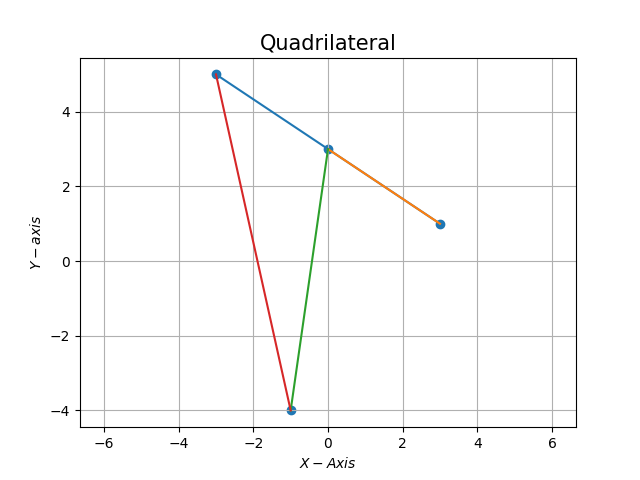
\includegraphics[width=\columnwidth]{figs/Figure_1.png}
			\caption{The points ABCD do not form a quadrilateral}
			\label{fig:7}
		\end{figure}

\end{document}
